\documentclass[12pt, letterpaper]{article}
\usepackage{graphicx}
\graphicspath{{Images/}}
\usepackage{subcaption} 
\usepackage[left=15mm,right=15mm,top=10mm,bottom=10mm,paper=a4paper]{geometry}
\usepackage{multirow}


\begin{document}
\begin{figure}[h]
	\centering
	\begin{minipage}{0.75\textwidth}
		\centering
		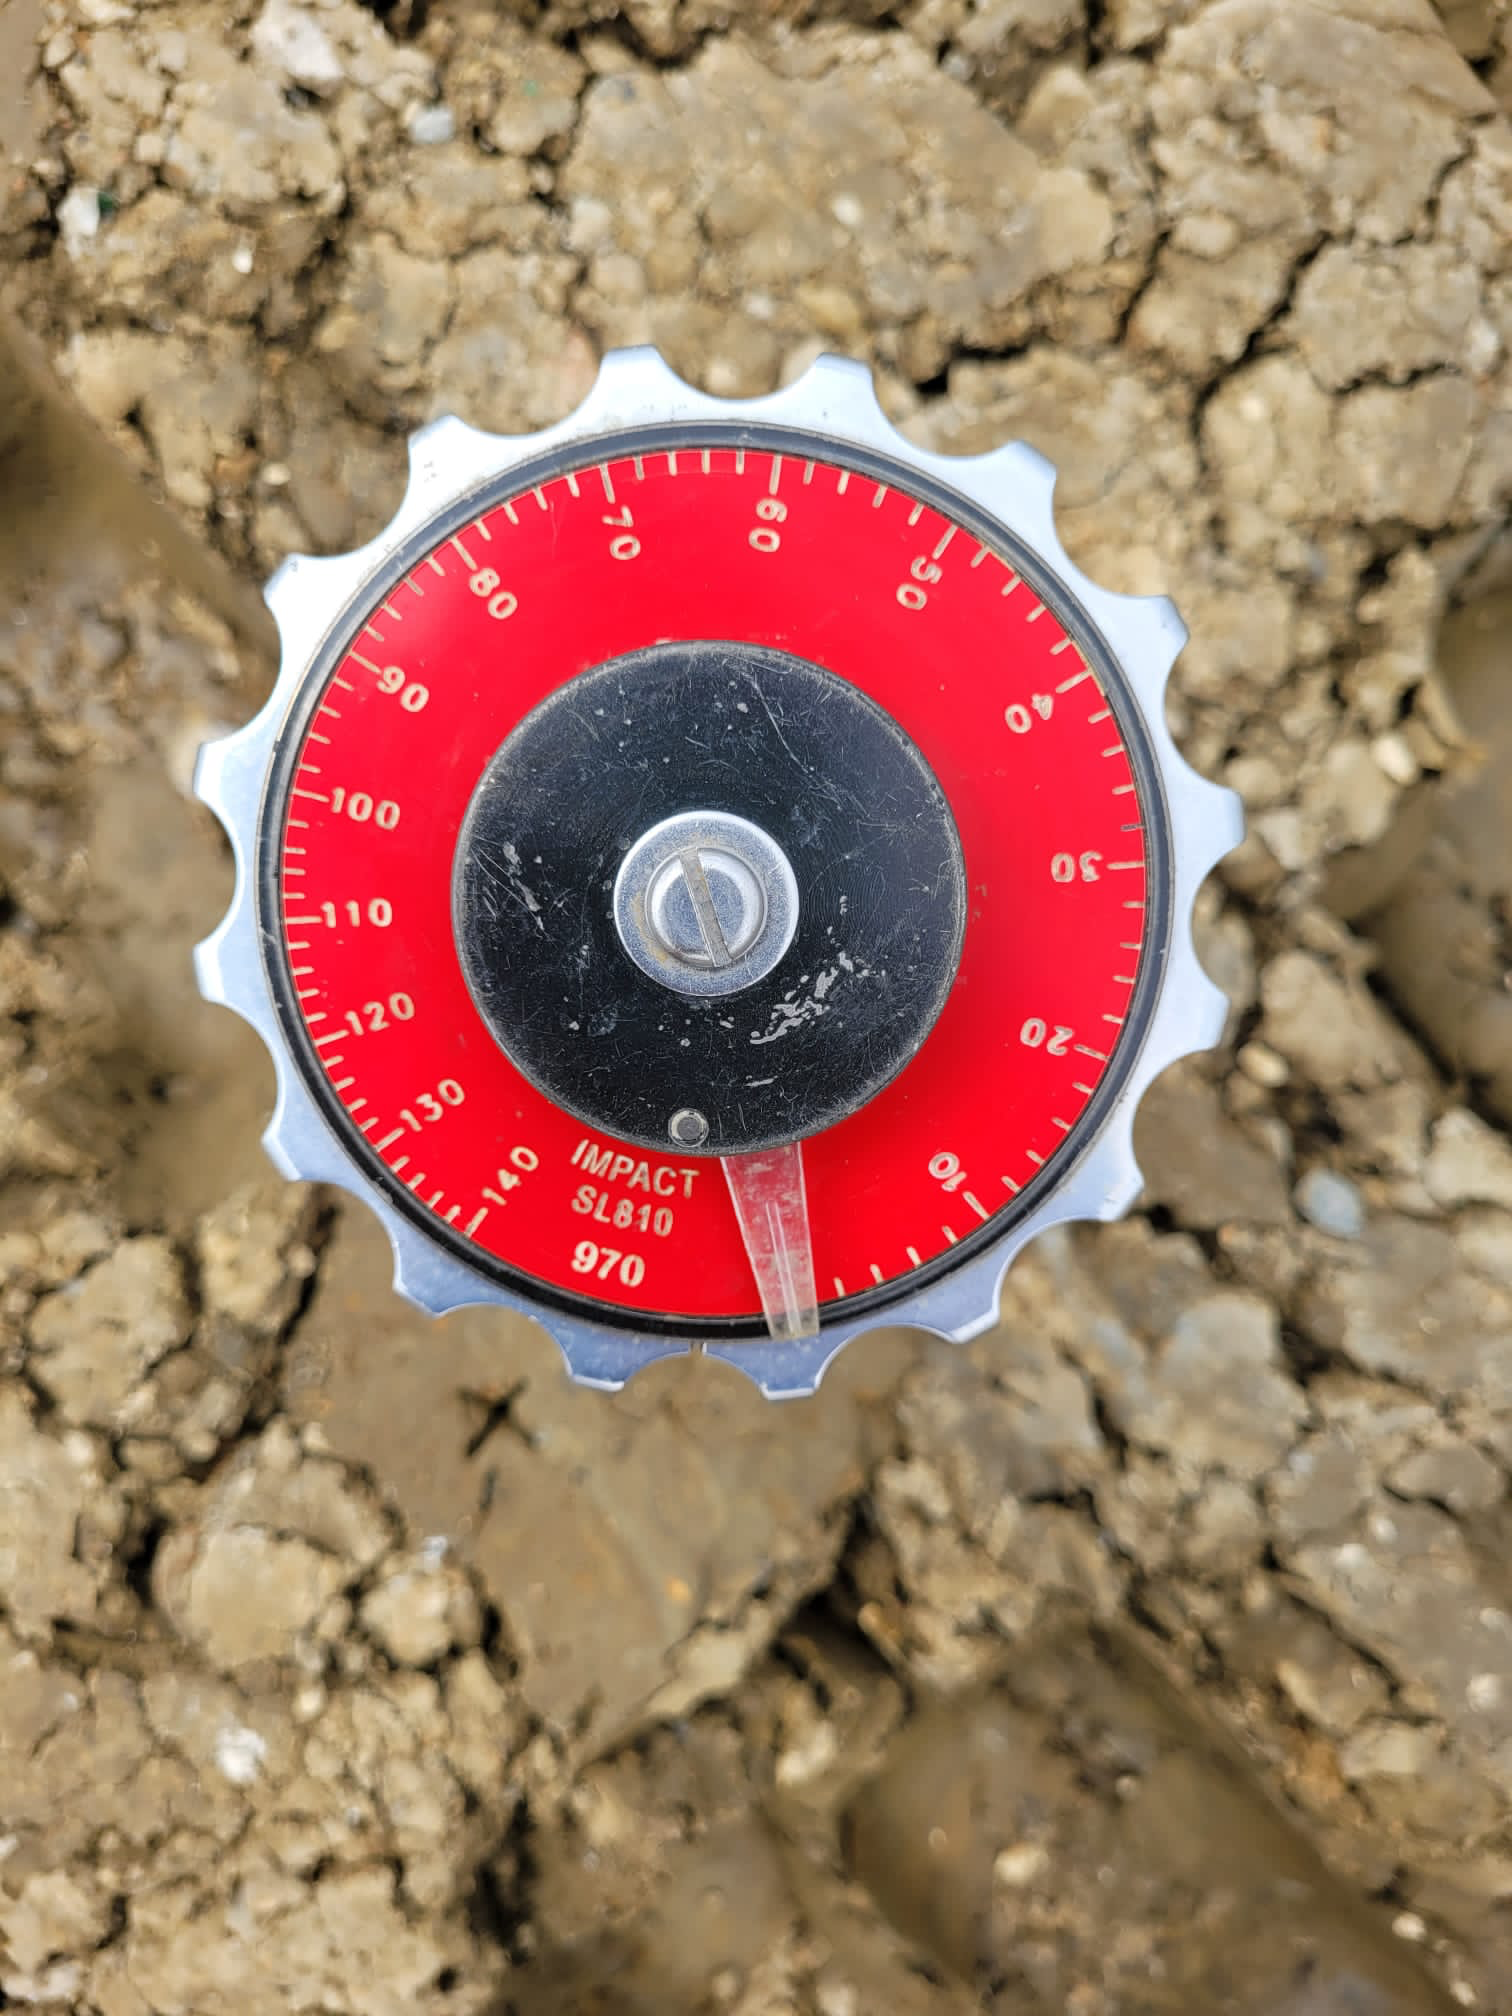
\includegraphics[height=0.33\textheight]{perm}
		\caption{Photo 1}
		\label{fig:dragon1}
	\end{minipage}

	\vspace{\baselineskip} 

	\begin{minipage}{0.75\textwidth}
		\centering
		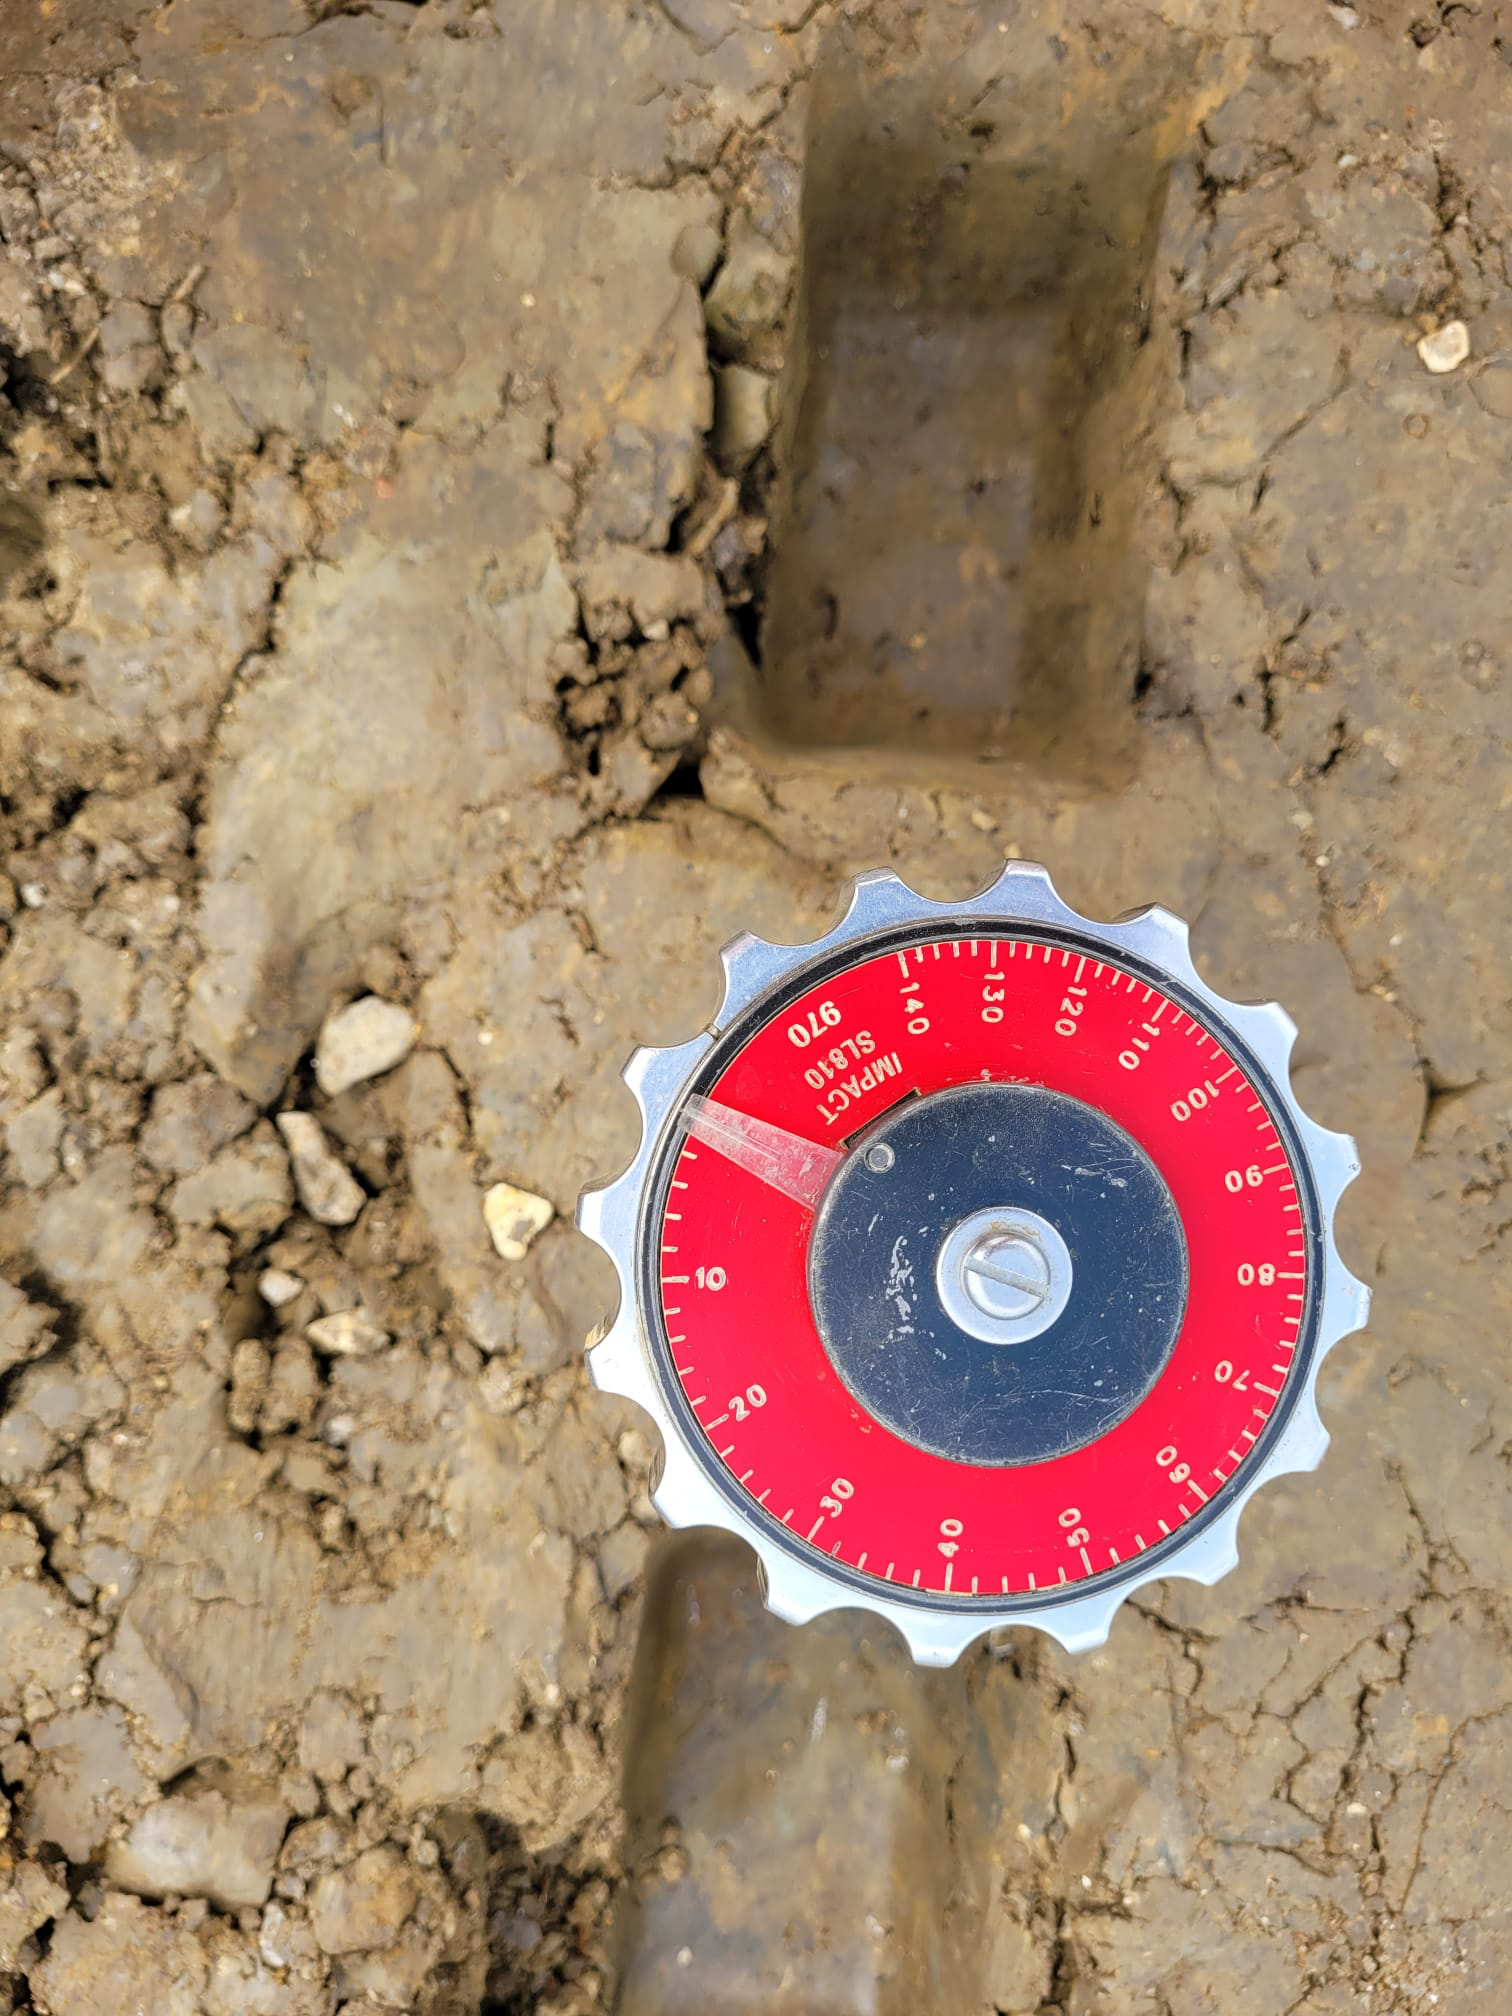
\includegraphics[height=0.33\textheight]{perm2}
		\caption{Photo 2}
		\label{fig:dragon2}
	\end{minipage}
	
\end{figure}

\begin{table}[h]
    \centering
    \scalebox{1}{ % Adjust the scaling factor as needed
        \begin{tabular}{|l|c|}
            \hline
            \multirow{2}{*}{Left Column} & Row 1, Right \\
            \cline{2-2}
            & Row 2, Right \\
            \hline
        \end{tabular}
    }
\end{table}

\end{document}